\documentclass{report}
\usepackage{arxiv, doi, graphicx, url, verbatim, multirow, colortbl, anyfontsize, hyperref}
\usepackage[english]{babel}
\usepackage[utf8]{inputenc}
\usepackage[T1]{fontenc}

\usepackage{csquotes}
\usepackage[backend=biber, style=apa]{biblatex}
\addbibresource{references.bib}

\usepackage[dvipsnames]{xcolor}

\usepackage{tikz}
\usetikzlibrary{calc}
\begin{document}
\pagestyle{empty}

\begin{tikzpicture}[overlay,remember picture]

% Background color
\fill[
black!2]
(current page.south west) rectangle (current page.north east);

% Rectangles
\shade[
left color=Dandelion, 
right color=Dandelion!40,
transform canvas ={rotate around ={45:($(current page.north west)+(0,-6)$)}}] 
($(current page.north west)+(0,-6)$) rectangle ++(10,1.5);

\shade[
left color=lightgray,
right color=lightgray!50,
rounded corners=0.75cm,
transform canvas ={rotate around ={45:($(current page.north west)+(.5,-10)$)}}]
($(current page.north west)+(0.5,-10)$) rectangle ++(15,1.5);

\shade[
left color=lightgray,
rounded corners=0.3cm,
transform canvas ={rotate around ={45:($(current page.north west)+(.5,-10)$)}}]
($(current page.north west)+(1.5,-9.55)$) rectangle ++(7,.6);

\shade[
left color=purple!80,
right color=blue!60,
rounded corners=0.4cm,
transform canvas ={rotate around ={45:($(current page.north)+(-1.5,-3)$)}}]
($(current page.north)+(-1.5,-3)$) rectangle ++(10,1);

\shade[
left color=red!80,
right color=red!80,
rounded corners=0.9cm,
transform canvas ={rotate around ={45:($(current page.north)+(-3,-8)$)}}]
($(current page.north)+(-3,-8)$) rectangle ++(15,1.8);

\shade[
left color=orange,
right color=Dandelion,
rounded corners=0.9cm,
transform canvas ={rotate around ={45:($(current page.north west)+(4,-15.5)$)}}]
($(current page.north west)+(4,-15.5)$) rectangle ++(30,2);

\shade[
left color=RoyalBlue,
right color=Emerald,
rounded corners=0.75cm,
transform canvas ={rotate around ={45:($(current page.north west)+(13,-10)$)}}]
($(current page.north west)+(13,-10)$) rectangle ++(15,1.5);

\shade[
left color=lightgray,
rounded corners=0.3cm,
transform canvas ={rotate around ={45:($(current page.north west)+(18,-8)$)}}]
($(current page.north west)+(18,-8)$) rectangle ++(15,0.5);

\shade[
left color=lightgray,
rounded corners=0.5cm,
transform canvas ={rotate around ={45:($(current page.north west)+(19,-5.65)$)}}]
($(current page.north west)+(19,-5.65)$) rectangle ++(15,1);

\shade[
left color=OrangeRed,
right color=red!80,
rounded corners=0.5cm,
transform canvas ={rotate around ={45:($(current page.north west)+(20,-9)$)}}] 
($(current page.north west)+(20,-9)$) rectangle ++(15,1);

% Sostituire con logo Politecnico molesto
\draw[ultra thick,black!2]
($(current page.center)+(2,1)$) -- ++(0,0cm) 
node[
midway,
right=-6.75cm,
text width=9cm,
align=center]
{
{
\includegraphics[width=.4\textwidth]{Logo_Politecnico_Milano.png}}
};

% Title
\node[align=center] at ($(current page.center)+(0,-5)$) 
{
{\fontsize{40}{50} \selectfont {{}}} \\[0.7cm]
{\fontsize{40}{50} \selectfont {{Ethics of Transportation}}} \\[0.5cm]
{\fontsize{40}{50} \selectfont {{Workshop portfolio}}} \\[1.5cm]
{\fontsize{15}{20} \selectfont \textcolor{black}{ \bf \underline{Group 1B}}}\\[10pt]
{\fontsize{15}{20} \selectfont \textcolor{black}{ \bf Alessandro Barbero (10536528)\quad Luca Cattaneo (10521219)\quad Mara Pegoraro (10629697)}}\\[10pt]
{\fontsize{15}{20} \selectfont \textcolor{black}{ \bf Jacopo Elia Pometto (10521596)\quad Giovanni Valtorta (10528573)}}\\[15pt]
{\fontsize{10}{10} \selectfont \textcolor{black}{ \bf {A.Y. 2021 - 2022}}}\\[0pt]
};
\end{tikzpicture}
\newpage
\chapter*{Abstract}
\pagenumbering{roman}
\begin{center}
This is a portfolio made for the course of \textit{Ethics for Transportation}, in the \textbf{Master of Science of Mobility Engineering} at \textit{Politecnico di Milano}.

The aim of this text is the practical analysis of the theoretical and ethical theories applied to the transportation sector. It consists of two parts: the collection of all the \textit{reports} written during the course and the final \textit{individual reflection} made by the authors.
\end{center}

\tableofcontents
\pagenumbering{arabic}

\part{Reports}
\chapter{VSD}
\begin{figure}[h]
\centering
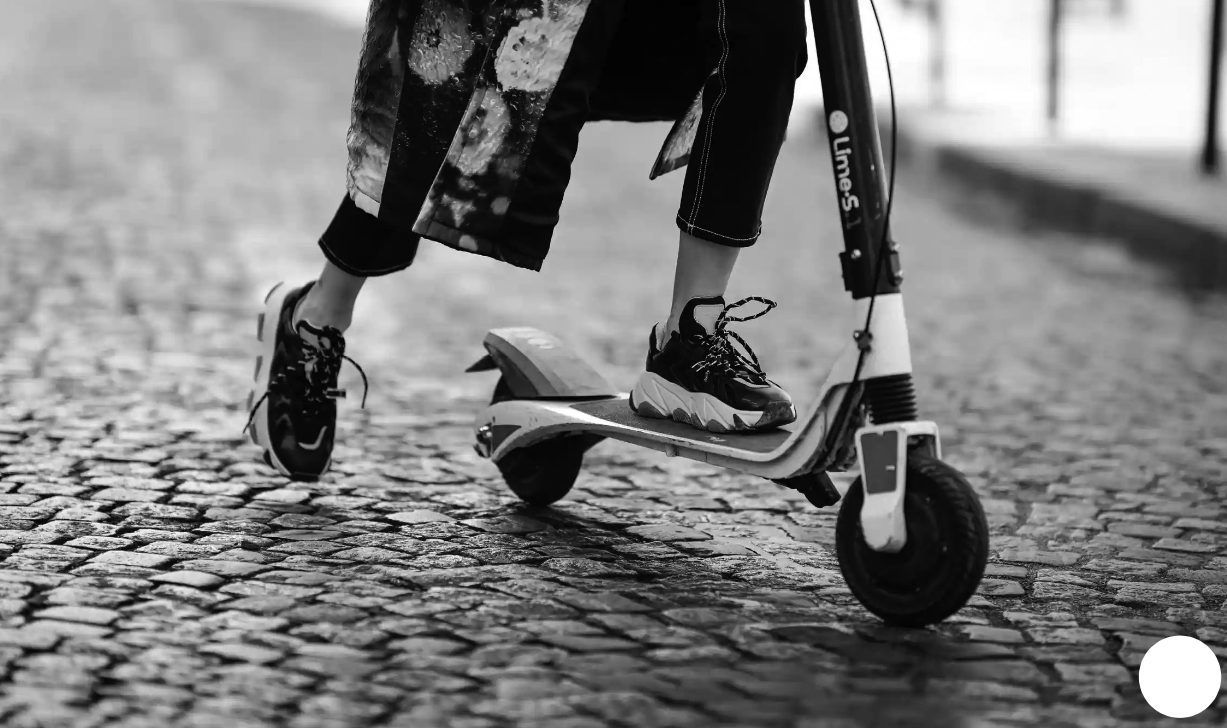
\includegraphics[width=0.8\textwidth]{Capitoli_Report/2.1_VSD.png}
\caption{\cite{vsdpic}}
\label{fig:vsd}
\end{figure}
\newpage
\pagestyle{plain}
\section{Introduction}
The case study regards the problem of e-scooters in urban context, critically reviewed using the \textit{Value Sensitive Design} method seen during the lesson. The stakeholder we selected is a \textit{pedestrian}, and we chose safety \textit{safety} as a value.

In the next table are listed the selected value, the norms and their design requirements:

\begin{table}[h]
\centering
\begin{tabular}{|l|l|l|}
\hline
\multicolumn{1}{|c|}{\textbf{Value}} & \textbf{Norms}                           & \textbf{Design requirements}        \\ \hline
\multirow{8}{*}{Safety}              & \multirow{2}{*}{Road rules}              & Use of separate lane                \\ \cline{3-3} 
                                     &                                          & Speed limitation                    \\ \cline{2-3} 
                                     & \multirow{2}{*}{Health defense}          & Recyclable components               \\ \cline{3-3} 
                                     &                                          & Low manufacturing emissions         \\ \cline{2-3} 
                                     & \multirow{2}{*}{Social responsibility}   & Insurance                           \\ \cline{3-3} 
                                     &                                          & Driving suitability certificate     \\ \cline{2-3} 
                                     & \multirow{2}{*}{Notability}              & Acoustic signaling                  \\ \cline{3-3} 
                                     &                                          & Visual signaling                    \\ \hline
\end{tabular}
\end{table}

\emph{(54 words)}

\section{Definition of \textit{Safety}}
Taking inspiration from the \textit{\cite{EBSafe}}, with safety we mean those activities whose aim is to minimize or to eliminate hazardous conditions that can cause bodily injury. We fall into two principal headings: occupational safety and public safety. When we talk about e-scooters we are in the public safety domain which contains all the policies that involve hazards at home, in travels and for recreational purposes.

We agreed with this definition because every pedestrian, not using an e-scooter, wants to be sure that he will not be harmed by the other riders when walking during his daily routine.

\emph{(100 words)}

\section{Possible conflict with other stakeholder’s interests and/or other values}
\subsection{Potential value tensions}
When dealing with safety for pedestrian, we could notice a value tension between walking people and e-scooter riders’ interests. As said before, feeling safe and sound from accidents for pedestrians would conflict with the necessity for riders to travel in a faster way and therefore exploiting walking lanes rather than the road. 

Another value tension can be noticed if we consider that people can use e-scooters also for fun, here considered as a value in contrast, again, with safety for pedestrians. In fact, the safety feeling of pedestrians can decrease in presence of riders that use the e-scooter not only for moving, but also as something to play with, doing dangerous maneuvers like going at high speed or making sudden turns and brakes.

Another point is that e-scooters, as well as many other vehicles, are not considered simply as means of transport: many people see them as status symbols. This insight could encourage some e-scooter users to a more superficial use of these vehicles, with negative impacts on pedestrians’ safety.

\newpage
\subsection{Possible solutions}
These issues could be tackled in different ways. One can be introducing dedicated lanes for e-scooters and speed limitations, together with some driving regulation. Also, it could be considered to spread awareness about the proper use of e-scooters and make citizens feel responsible for their own actions on the streets. A stricter solution could be the implementation of a more severe control on users, giving fines to those who do not comply with the correct behavior. A more practical aspect could be the introduction of visual and acoustic signaling.

Whether these measures couldn't be applied, pedestrian’s value of safety should be favored, since they are the weaker stakeholder on the road, in terms of velocity of motion and protection measures and, moreover, riders could anyway travel on road lanes and not on the sidewalk.

\emph{(307 words)}

\section{Utility of VSD for mobility engineers}
\label{vsd}
We think that Value Sensitive Design is maybe one of the most important things to be kept in mind in our work as Mobility Engineers. Being that our MSc offers an interdisciplinary approach towards the broad theme of mobility, it is vital that all different perspectives are considered. Mobility will be a great challenge in the future, either if you consider it as moving 8 billion people from A to B in the most sustainable way possible, or as a service you are offering as a company. All different stakeholders’ opinions and values need to be considered even if this means complicating the analysis. Value tensions and criticalities need to be resolved in any possible way, being mobility something that concerns everyone.

\emph{(122 words)}

\emph{(527 total words)}

\begin{comment}
\newpage
\begin{thebibliography}{99}

\bibitem[EB, 2017]{p1}  
Encyclopaedia Britannica (2017)

\textit{Safety} Accessed on October 09, 2021

\url{https://www.britannica.com/topic/safety-condition}

\bibitem[VSD, 2015]{p2}
Davis, J., \& Nathan, L. P. (2015)

\textit{Value sensitive design: Applications, adaptations, and critiques.}

\textbf{In Handbook of Ethics, Values, and Technological Design: Sources, Theory, Values and Application Domains}

\bibitem[Watkins, 2021]{p3}
Watkins, K. E. , (2021)

\textit{Using value sensitive design to understand transportation choices and envision a future transportation system.}

\textbf{Ethics and Information Technology, 23(1)}

\end{thebibliography}

\textit{Document write with \LaTeX. Template founded on Overleaf} (\textbf{Copyright (c) 2020 George Kour}).
\end{comment}
\newpage
\chapter{Justice}
\begin{figure}[h]
\centering
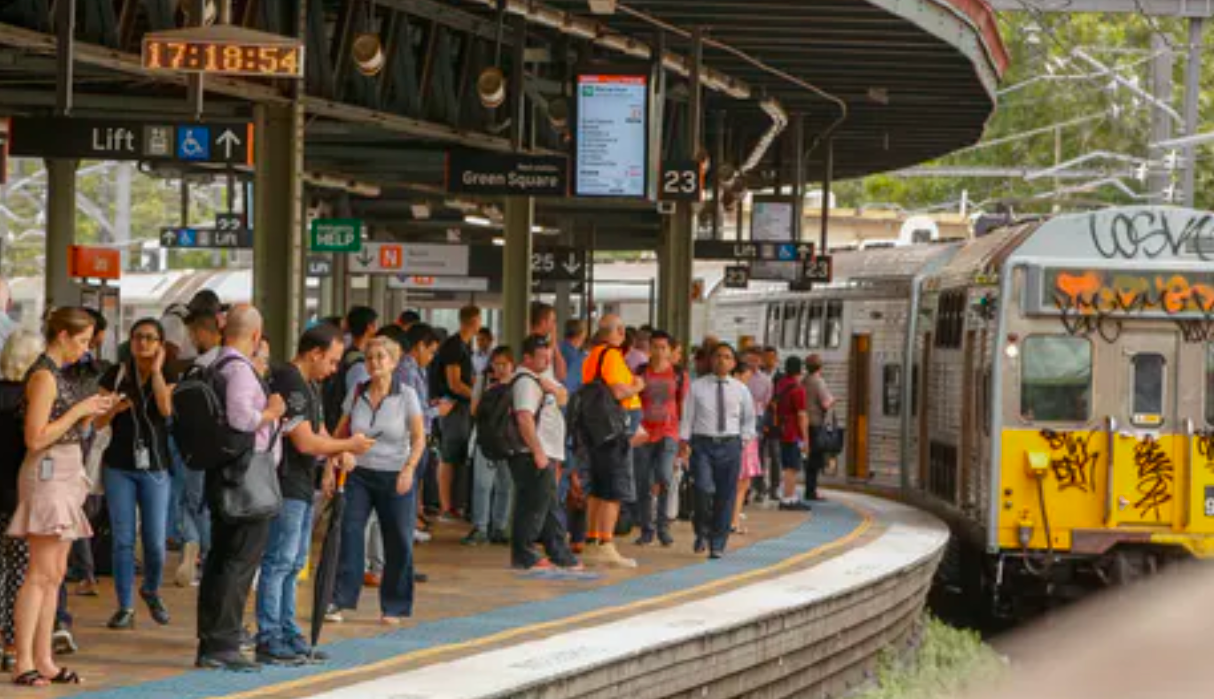
\includegraphics[width=0.8\textwidth]{Capitoli_Report/3.1_Justice.png}
\caption{\cite{picjustice}}
\label{fig:justice}
\end{figure}
\newpage
\section{Introduction}
The case study regards the comparison of two possible theories to apply in order to decide whether to build a new highway bridge or the BART tunnel in the San Francisco Bay Area. The approaches we selected are \textit{utilitarianism} and \textit{libertarianism}.

\emph{(41 words)}

\section{What are the most important implications of using the selected approaches in the choice between the BART tunnel and the highway bridge?}

{\em{\bfseries Libertarians}} think that people are able to pursue their best interests when left free to act. Consequently, any intervention of the authority should be limited; moreover, in a libertarian society, infrastructures and services would be run completely by private actors pursuing only their personal income, so the most suitable project would be the highway bridge. In fact, it is much cheaper than the BART, resulting in a lower CAPEX for the (private) construction company and it is also the alternative that would have a greater market share. This solution allows to apply fares for the transit, so with the assumption that the two infrastructures would generate the same income, a less expensive solution would create more profit, being the alternative that a company in a libertarian system would naturally choose. Obviously this would not take into account the poorest people, who are unable to afford the expenses, leading to a non-optimal distribution of opportunities and generating an improved quality of life only for a minority of the population. We can understand that for libertarians, only taxpayers and contributing people’s opinion should be taken into account. 

{\em{\bfseries Utilitarians}} instead aim to maximize the total benefit quantified using economic terms, considering as equally important everyone’s opinion on the issue. The counter effect of this strategy is the concentration only on necessities shared by the majority of people or even worse, only on few people able to obtain great improvements, counterbalancing eventual relative losses of the rest of the population. According to this approach, the most suitable project would still be the car bridge, since the majority of people (72\%) seems to prefer the private transport. Again, the most disadvantaged citizens would anyway be penalized, needing to afford a car to get access to the service.

{\em{\bfseries In general terms}}, consequences of a libertarian approach risk to be harsher with respect to the utilitarian ones, because they are inherently unfair, distributing opportunities unequally among the population and preventing disadvantaged people from flourishing. Utilitarianism that is still a non-optimal solution, takes someway into account everyone’s need and tries to pursue a generalized development, even if often at minorities' expenses. Another good point in favor of utilitarianism, is the evaluation and quantification of bad consequences of policies assuring a higher benefit and so, theoretically, the possibility to refund the underprivileged, that could become convenient if misery begins to widespread, threatening even majorities' well being.

\emph{(399 words)}

\section{What are the most important differences between these two theories of justice applied to this case in terms of:}
\subsection{Practicality}
The utilitarian approach addresses how to distribute the greatest good among all the members and it is the basis of the {\rmfamily Cost Benefit Analysis} (\texttt{CBA}), that analyzes costs and benefits for each alternative to prioritize the most convenient ones, allowing a quantifiable control of the different objectives. Practicality can be quantified with different indicators that need to be maximized in order to produce the greatest utility. 

Libertarianism instead does not allow any external intervention, emphasizing the individual freedom and the financial feasibility. This leads towards the solution that is the most economically convenient, but could not be the one that is shared by the majority of the users, nor the socially optimal one.

\subsection{Fairness}
From this point of view, the most useful approach is utilitarianism because, despite it can address only the activities used by majoritarian classes and eventual bad externalities will fall only on minoritarian classes, it is also true that these problems can be solved by addressing in \texttt{CBA} those externalities. Instead, libertarianism will solve no problem in case of market failures. 

An example, remaining in the case of infrastructure investment, can be the case of internet home connection in Italy. Due to a free market libertarian approach, we have towns served only by \texttt{ADSL} from a single infrastructure operator, because they have less users of the internet service, while other cities are served with \texttt{FTTH} with more than one infrastructure operator, being easier for them to make a profit.

\emph{(241 words)}

\emph{(681 total words)}

\begin{comment}
\newpage
\begin{thebibliography}{99}

\bibitem[Justice, 2017]{p2}
Pereira et al. (2017)

\textit{Distributive justice and equity in transportation.}

\textbf{Transport Reviews, 37(2)}

\bibitem[Investment Decisions, 2020]{p3}
Kevin DeGood (2020)

\textit{Infrastructure Investment Decisions Are Political, Not Technical.}

\textbf{Center for American Progress}

\end{thebibliography}
\textit{Document write with \LaTeX. Template founded on Overleaf} (\textbf{Copyright (c) 2020 George Kour}).
\end{comment}
\newpage
\chapter{Safety}
\begin{figure}[h]
\centering
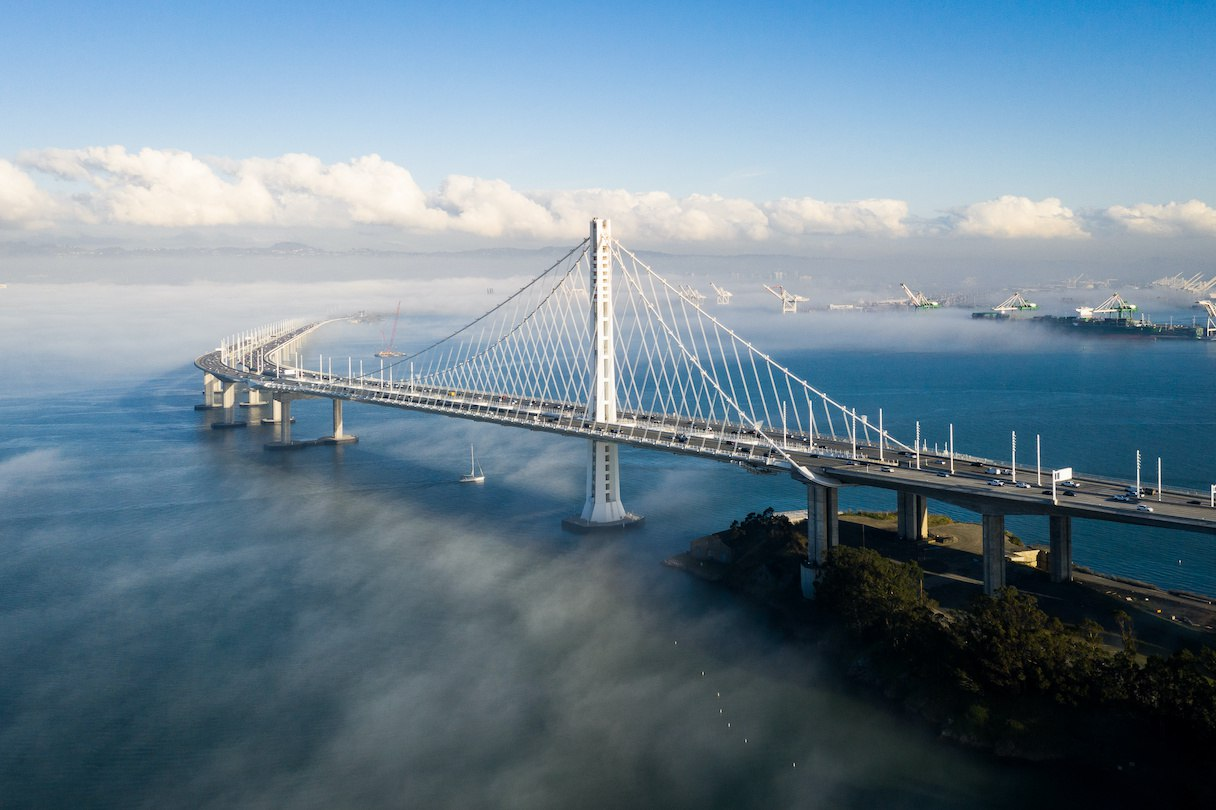
\includegraphics[width=0.8\textwidth]{Capitoli_Report/4.1_Safety.png}
\caption{\cite{picsafety}}
\label{fig:safety}
\end{figure}
\newpage
\section{Introduction}
The case study regards the discussion of a \textit{fictional case of liberty limitation techno-regulation} in transportation, which is the implementation of the \textbf{Intelligent Decibel Lowering Engine Restrainer} (IDLER) on all new motorcycles. This is a device that allows to automatically limit the engine's maximum RPM, in order to reduce the (excessive) emitted noise in certain locations, thanks to a GPS installed on board.

\emph{(65 words)}

\section{What are the two most convincing arguments \textit{in favor of obligating} the implementation of IDLER, in your opinion?}
\subsection{Public nuisance}
On certain roads or in urban centers there can be a very intense traffic of motorcycles, since they could be near places that are very attractive for motorcyclists: roads bordering a lake or mountain passes are all places where it can be very pleasant to ride, as they are very engaging from the driver's point of view. For this reason, the constant passage of motorcycles could become very annoying for the inhabitants of those places and disturb their quietness, especially during the weekends. Therefore, as there are already regulations that prohibit to honk in the cities or to make noises late at night, the introduction of a device such as IDLER could be considered to better preserve and guarantee public peace. In addition, WHO classifies as "harmful" every sound above 75 dB, and almost all bikes can go beyond this limit.

\subsection{Pollutant emissions}
When going at high speed and high RPM, the engine produces lots of pollutant emissions, so its introduction could also help from the point of view of reducing them, especially in the city center, where this problem is more present than other places.

\emph{(198 words)}

\section{What are the two most convincing arguments \textit{against obligating} the implementation of IDLER, in your opinion?}
\subsection{Limited driving experience}
Usually, high-performance and sport motorcycles, with a particularly loud exhaust sound, are mainly purchased by enthusiasts to use them specifically on the roads mentioned above: in these cases, sound plays an active role in driving involvement, so its attenuation or elimination could be seen as a limitation to one's passion and, consequently, to one's freedom.

\subsection{Low flexibility in case of emergency}
Other problems may arise if the driver needs to move faster than the IDLER allows, due to a sudden need or emergency. As an extreme consequence, this could also lead to people not buying these type of vehicles, decreasing the  motorcycles' selling. Another aspect to be considered is the nature of the motorcycle itself. To negotiate a curve, a motorbike of any sort needs a given speed to generate the forces that make the leaning equilibrium possible. If, for any reason (GPS malfunctioning, bad tuning of the interested zones, IDLER malfunctioning and similar), the IDLER would cut power while curving, this can lead to a loss of control and eventually even to a crash.

\emph{(172 words)}

\section{Considering the previous arguments, are you in favor or against the obligatory implementation of IDLER? And \textit{why}?}
The implementation of some device to reduce acoustic pollution is something that any motorcyclist would approve, if he/she was the one suffering the discomfort. What makes IDLER not the best solution, however, is the lack of controllability; GPS is not an accurate system, so errors in the position estimation can lead to dangerous situations.

A solution that can make the IDLER's philosophy applicable is to couple it with some ad hoc legislation and infrastructure.
One example can be the implementation of an IDLER that switches on based on signals coming from sensorized roads only in proximity of points of interest (like hospitals and schools). These conditions must be adequately marked by signage, so that the rider is prepared for the fact that the bike will suddenly lose power. Another aspect to consider is personal responsibility. Motorcycles tend to produce the most noise when the engine RPMs are high and that, in most of real-life scenarios, corresponds to the bike going fast. By introducing speed limits, combined with some effective speed radars targeted to specific zones like the aforementioned, IDLER will maybe not even be necessary.

In conclusion, IDLER is an interesting solution; it makes riders renounce to a trivial pleasure like the sound of a high revving bike for a great public good. However, how to apply this concept is something that needs some further analysis to give the best solution.

\emph{(213 words)}

\emph{(549 total words)}

\begin{comment}
\begin{thebibliography}{99}

\bibitem[Fahlquist, 2009]{p1}
Fahlquist, J. N. (2009)

\textit{Saving lives in road traffic-ethical aspects.}

\textbf{Journal of Public Health, 17(6)}

\bibitem[Smids, 2018]{p2}
Smids, J. (2018)

\textit{The moral case for intelligent speed adaptation.}

\textbf{Journal of Applied Philosophy, 35(2)}

\end{thebibliography}

\textit{Document write with \LaTeX. Template founded on Overleaf} (\textbf{Copyright (c) 2020 George Kour}).
\end{comment}
\newpage
\addtocontents{toc}{\vspace{4em}}
\chapter{Privacy}
\begin{figure}[h]
\centering

\includegraphics[width=0.8\textwidth]{Capitoli_Report/5.1_Privacy.png}
\caption{\cite{picprivacy}}
\label{fig:privacy}
\end{figure}
\newpage
\section{Introduction}
The case study regards the connection between the philosophical analysis from the last workshop to ethical design, practicing the translation from the conceptual to the practical and viceversa. The analysis is based on the norms of appropriateness and of distribution defined by \textbf{Zimmer} \cite{Zimmer2005SurveillanceTechnologies}. 
\begin{table}[h]
\centering
\begin{tabular}{|c|l|l|}
\hline
\textbf{Value}                                             & \multicolumn{1}{|c|}{\textbf{Norms}}                                                                                                                            & \multicolumn{1}{|c|}{\textbf{Design requirements}}                                                                                              \\ \hline
\multicolumn{1}{|c|}{\multirow{12}{*}{\textbf{Privacy}}}   & \multicolumn{1}{l|}{\multirow{2}{*}{A1: acquired data contain only the image}}                                                                                 & \multicolumn{1}{l|}{\multirow{2}{*}{No metadata for images taken from passengers}}                                                               \\
\multicolumn{1}{|c|}{}                                     & \multicolumn{1}{l|}{}                                                                                                                                           & \multicolumn{1}{l|}{}                                                                                                                           \\ \cline{2-3} 
\multicolumn{1}{|c|}{}                                     & \multicolumn{1}{l|}{\multirow{2}{*}{\begin{tabular}[c]{@{}l@{}}A2: don't merge images \\\qquad with data from other sources\end{tabular}}}                     & \multicolumn{1}{l|}{\begin{tabular}[c]{@{}l@{}}Impossibility of making query \\ in other dataset of the instrument\end{tabular}}               \\ \cline{3-3} 
\multicolumn{1}{|c|}{}                                     & \multicolumn{1}{l|}{}                                                                                                                                           & \multicolumn{1}{l|}{\begin{tabular}[c]{@{}l@{}}Database with only photo \\ of the inhabitants\end{tabular}}                  \\ \cline{2-3} 
\multicolumn{1}{|c|}{}                                     & \multicolumn{1}{l|}{\multirow{2}{*}{\begin{tabular}[c]{@{}l@{}}A3: renew resident images \\ \qquad in the database at regular time\end{tabular}}}                & \multicolumn{1}{l|}{Automatic reset of image dataset}                                                                                           \\ \cline{3-3} 
\multicolumn{1}{|c|}{}                                     & \multicolumn{1}{l|}{}                                                                                                                                           & \multicolumn{1}{l|}{\begin{tabular}[c]{@{}l@{}}Acquire the photo provided \\ for the Identity card\end{tabular}}                         \\ \cline{2-3} 
\multicolumn{1}{|c|}{}                                     & \multicolumn{1}{l|}{\multirow{2}{*}{D1: data not shared}}                                                                                                       & \multicolumn{1}{l|}{\multirow{2}{*}{Local dataset}}                                                                                             \\
\multicolumn{1}{|c|}{}                                     & \multicolumn{1}{l|}{}                                                                                                                                           & \multicolumn{1}{l|}{}                                                                                                                           \\ \cline{2-3} 
\multicolumn{1}{|c|}{}                                     & \multicolumn{1}{l|}{\multirow{2}{*}{D2: data kept only for limited amount of time}}                                                                             & \multicolumn{1}{l|}{\multirow{2}{*}{\begin{tabular}[c]{@{}l@{}}Automatic reset of the memory\\  used to store acquired data\end{tabular}}}     \\
\multicolumn{1}{|c|}{}                                     & \multicolumn{1}{l|}{}                                                                                                                                           & \multicolumn{1}{l|}{}                                                                                                                           \\ \cline{2-3} 
\multicolumn{1}{|c|}{}                                     & \multicolumn{1}{l|}{\multirow{2}{*}{\begin{tabular}[c]{@{}l@{}}D3: if data required by authority \\ \qquad only with mandate (according to law)\end{tabular}}} & \multicolumn{1}{l|}{\multirow{2}{*}{\begin{tabular}[c]{@{}l@{}}End to End cryptography \\ between the camera and the storage/analysis system\end{tabular}}} \\
\multicolumn{1}{|c|}{}                                     & \multicolumn{1}{l|}{}                                                                                                                                           & \multicolumn{1}{l|}{}                                                                                                                           \\ \hline
\end{tabular}
\label{tab:my-table}
\end{table}
\emph{(48 words)}

\section{Conceptualization of privacy}
\textbf{Privacy} is the condition in which all the entities not involved in yourself interest, or who did not receive your own acceptance, \textit{are deprived from accessing your personal data, such as habits and living area}. To do so, data collection from systems must always respect \textbf{contextual integrity} and its norms:
\begin{itemize}
    \item In \textbf{norms of appropriateness}, this concept declines in the given context considering the collection only of the amount of data that are needed to perform facial matching, and not any other information.

    \item \textbf{Norms of distribution} may instead concern the fact that the data collected must not be shared with other entities outside of the bridge automatic toll system, to prevent eventual loss of users’ privacy.
\end{itemize}

\emph{(115 words)}

\section{Does the solution present privacy concerns? Discuss for each of Reiman’s risks of privacy loss.}

\paragraph{Extrinsic Loss of Freedom}
It is defined as \textit{"all those ways in which lack of privacy makes people vulnerable to having their behavior controlled by others"}.

In this case, the risk is minimized by the fact that data are saved locally. But, we still could have some conditioning on people's travel habits: in fact, they could feel observed only because of the presence of cameras, like drivers that slow down approaching a speed trap, even though they know it is turned off. By the way, this risk could be considered acceptable, especially if we consider that the population will be properly informed about the functioning of the system and of the data collected.
\newpage
\paragraph{Intrinsic Loss of Freedom}
According to Reiman, it is the \textit{"ways in which denial of privacy limits people's freedom directly"}.

According to that, we do not face out any problems with the only exception of the presence of the toll system. Indeed, it limits the privacy of the single citizen, being forced to share his/her image to be recognizable and to have free access to the island. However, this intrinsic limitation of freedom is negligible especially for residents, since they are not required to pay the fee.

\paragraph{Symbolic Risk}
In the conception of the panopticon, it is defined as \textit{"a kind of draining off our individual sovereignty away and outside of us into a single center"}.

In the present case, this risk does not seem to be relevant, in relation to the previously mentioned requirements and to the control, that is limited only to that specific geographical location. Nevertheless, diffused control on travel data could be a problem, because it could preclude individuals from their authority to withdraw from scrutiny of others.

\paragraph{Psycho-Political Metamorphosis}
Reiman, talking about the development of the panopticon states that, when continuously observed, \textit{individuals tend to lose their peculiarities and behave the same, with a loss in the different shades of personalities}.

We think that this consideration, however, does not apply to the implementation of this solution: the control is performed only for the sake of making people respect a rule and the data is kept locally for a short time. So, this technology does not collect enough information to condition people's psychology.

\emph{(359 words)}

\emph{(522 total words)}

\begin{comment}
\begin{thebibliography}{99}

\bibitem[Privacy, 2017]{p1}
Reiman, J. H. (2017)

\textit{Driving to the panopticon: a philosophical exploration of the risks to Privacy Posed by the Highway Technology of the future.}

\textbf{Privacy, 11(1)}

\bibitem[Ethics and Information Technology, 2005]{p2}
Zimmer, M. (2005)

\textit{Surveillance, privacy and the ethics of vehicle safety communication technologies.}

\textbf{Ethics and Information Technology, 7(4)}

\end{thebibliography}

\textit{Document write with \LaTeX. Template founded on Overleaf} (\textbf{Copyright (c) 2020 George Kour}).
\end{comment}
\newpage
\chapter{Risk}
\begin{figure}[h]
\centering

\includegraphics[width=0.8\textwidth]{Capitoli_Report/6.1_Risk.png}
\caption{\cite{picrisk}}
\label{fig:risk}
\end{figure}
\newpage
\section{Introduction}
The case study consists in the discussion of our position regarding the acceptability of the risks imposed by autonomous vehicles to vulnerable road users. This will be performed using the five ‘factors’ for the acceptability of risk presented in the lecture as a guiding structure.

The goal is \textit{to try to come to a clear conclusion} as to whether we think the risks to vulnerable road users are acceptable or not and, if that would not be possible, we will indicate why it is difficult or what would be necessary to be able to make the determination. We will start from the assumption that \textbf{while overall traffic safety significantly increases with the introduction of autonomous vehicles, safety for some vulnerable road users actually decreases slightly}.

\emph{(125 words)}

\section{Discussion}
\paragraph{The size of the risk}
To discuss about the size of this risk, two different views will be presented: a relative and an absolute one.

Talking about the relative size, of course in some car-oriented countries like the USA, the slight increase of risk to cyclists can be considered negligible looking at the great benefit that autonomous cars will give. However, in some other countries like the Netherlands, where cycling has an overall modal share of $27\%$ (\cite{enwiki:1057840626}), the weight of this change will be greater.
On the other hand, looking at this risk in absolute terms, considering the pretty straightforward fact that a cyclist is a person that wants, like a car user, to be safe during her/his trip, the size of this risk is something not negligible.

\emph{(126 words)}

\paragraph{The availability of alternatives with lower risk}
Considering that an increase in risk, however small, is not negligible, several alternatives are available which could help to reduce the risk for vulnerable road users, or at least to keep it at the same current level.

For example, we could think about the introduction of a road infrastructure that physically divides drivers from cyclists and pedestrians, reducing the number of interactions between them and consequently the number of accidents, thus increasing overall safety. But a solution of this type introduces non-negligible disadvantages, such as the time and money required for its implementation. Therefore, in evaluating the possible use of alternative solutions, it is necessary that all the different stakeholders are willing to sacrifice something to favor the safety of the other party and, ultimately, the introduction of autonomous driving itself.

\emph{(132 words)}

\paragraph{Whether/to what extent the benefits outweigh the risks}
Utilitarians would argue that, as car drivers represent the majority of traffic users, an increase in their safety at the expense of vulnerable road users would be justifiable. However, this is probably a too trivial approach to decide whose safety has to be sacrificed. Also, it is conventionally believed that vulnerable users are the ones that should be more protected on the road.

Considering these aspects, the benefits of autonomous vehicles would outweigh the risks only in the case where car users’ deaths and injuries would decrease so much, that a slight worsening in vulnerable users’ conditions would be acceptable.

\emph{(100 words)}
\newpage
\paragraph{The degree of informed consent (or equivalent) for the risks}
In theory, a technical development leading to an increased safety for car-drivers would easily find their consent while, on the contrary, this would not happen for vulnerable road-users. But car-drivers could also travel as vulnerable users and many pedestrian could drive their cars, so not necessarily all car-drivers would agree for a solution like that and vice versa.

Some people, like elders and disabled, cannot avoid being vulnerable, so their consent should be kept in consideration more attentively. But, since this measure would affect positively the whole society, only a very wide aware opposition of such stakeholders should influence the putting in place of this measure.

(110 parole)

\paragraph{The fair distribution of the benefits and risks}
The distribution of benefits and risks can rarely be fair. This is due to the impossibility to reach always the optimal solution; we will need to find a compromise, otherwise we will be stopped. This process will favor the categories with greater influence in the decision-making process.

In this case, the vulnerable road user will necessarily reach a compromise to avoid a riskier approach. At the same time, the users of autonomous vehicles will reach a compromise accepting some risks to avoid a stop of the usage of autonomous vehicle. The distribution of benefits and risks both depends on how much influence the different parties have in society, making the process unfair.

\emph{(113 words)}

\section{Conclusion}
Summarizing what has been said, the imposition of a higher risk for already vulnerable users is hardly acceptable. By the way, before coming to an exhaustive conclusion, some other considerations must be done. It must be kept into account that a more performing traffic flow would lead to significant benefits for the whole society: more effective services, less rescue time for emergency vehicles, less pollutant emission and other improvements.

We can understand that there would be many aspects that would counterbalance the increased risk when considering the vulnerable users welfare. So, to make a choice, we would need data about lives of people that would be saved thanks to those "externalities" and also how to consider other well being improvements indicator, such as economic savings, higher quality of life and similar.

\emph{(131 words)}

\emph{(700 total words)}

\begin{comment}
\begin{thebibliography}{99}

\bibitem [1]{p1}

Wikipedia contributors.

\textit{Cycling in the Netherlands.}

\href{https://bit.ly/3pvCNY7}{\textbf{Wikipedia, The Free Encyclopedia}} Accessed on 4th December 2021.

\bibitem [Hayenhjelm, 2012]{p2}

Hayenhjelm, M., \& Wolff, J. (2012).

\textit{ The Moral Problem of Risk Impositions: A Survey of the Literature.}

\textbf{European Journal of Philosophy}, 20(S1), e26–e51.

\end{thebibliography}
\end{comment}
\newpage
\chapter{Responsibility}
\begin{figure}[h]
\centering
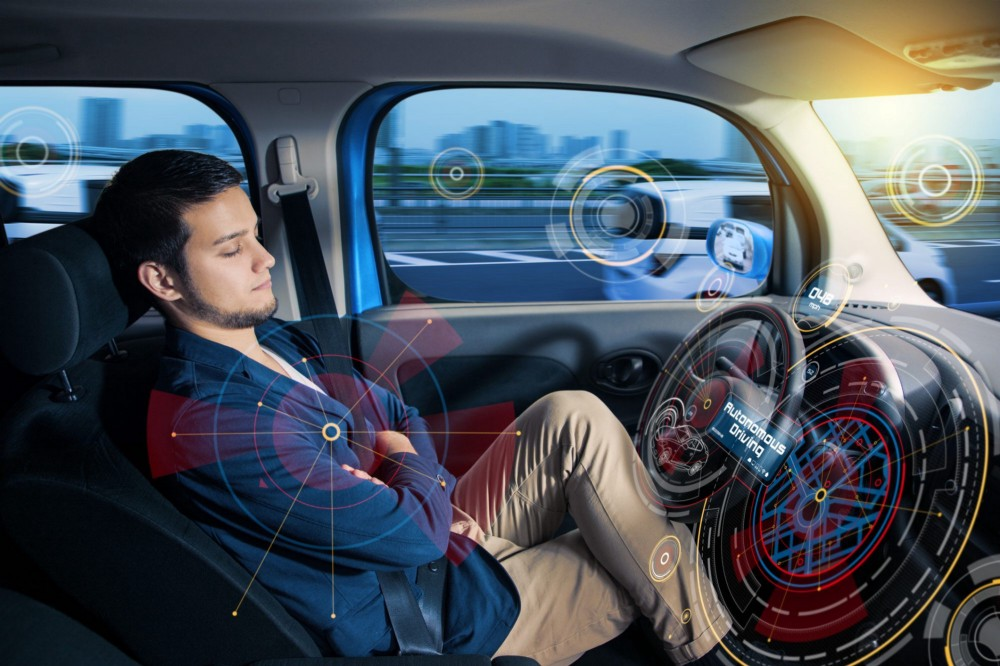
\includegraphics[width=0.8\textwidth]{Capitoli_Report/7.1_Responsibility.png}
\caption{\cite{picresponsibility}}
\label{fig:responsibility}
\end{figure}
\newpage
\section{Introduction}
The case study's objective is to revisit one of the transportation technologies previously discussed in the course through the lens of responsibility theory: the technology we decided to discuss is the \textbf{Intelligent Speed Adaptation} (ISA); it is \textit{a device that automatically limit the speed of a vehicle based on GPS signal or other techniques}. It is advertised that \textbf{its installation can be beneficial for reducing accidents and deaths on the road}.

The two types of responsibility that we think will change the most due to its introduction are \textbf{accountability} and \textbf{moral culpability}.

\emph{(92 words)}

\section{Discussion}
\subsection{Do you think that these changes are problematic? Propose at least two recommendations for improving the responsibility situation.}

We think the introduction of \textbf{ISA} would have effects on the responsibility in terms of \textbf{accountability} and \textbf{moral culpability}. The former is here intended as \textit{"the obligation to explain something that has happened and one's role in its occurrence"}, while the latter means \textit{"being open not only to requests for explanation but also to stronger social and legal responses"}. ISA would ideally be a device that runs continuously in background on the vehicle and so, describing a possible use case, we can consider a situation in which the driver is simply used to going flat-out all the time, letting ISA manage the speed of the car. \textit{But what if ISA fails?}

It could also mean that the driver could be able to overcome the speed limit, without even realizing it. In case this behavior results in the driver hitting a pedestrian, should the \textbf{responsibility} lie with the driver or with the system manufacturer/programmer, who did not manage to produce it as fail proof?

It could be argued that the \textbf{accountability} is totally to be attributed to the driver, who did not respect the limit; but what if he/she was not even realizing his/her wrongdoing, because of the wrong habits of putting all the trust of staying within the limits in the ISA system?

Also, \textbf{culpability} is something that needs to be analysed in the sense that, if the driver is able to use ISA in the way already described, the system is the only barrier that prevents the user from having the undesired behavior of going over the limits. Fallen that barrier, the user is not even realizing what he/she is doing. Both those aspects need to be addressed to define some clear \textit{responsibility boundaries}. One solution can be putting some indicators in the dashboard to inform the driver about the fail of the ISA, or to make it adaptive, so that also the pedal has some feedback to regulate the speed.

\textit{Accountability gaps} could be avoided by the policymaker, that should arrange strict regulation for the production of the ISA. For instance, the manufacturer should provide documentation that simplifies the comprehensibility in case of failures of the device, in order to potentially allocate responsibility also to the producer.

\textit{Culpability gaps} could be avoided ensuring a coordination between the ethical, legal, sociological, and technical field. This could be implemented creating professional profiles characterized by broad-spectrum knowledge in these disciplines, allowing an effective communication between very different contexts and avoiding scapegoating mechanisms.

\emph{(417 words)}
\newpage
\subsection{Would this new situation be helped, in terms of responsibility attribution and/or of institutional organization, by increased collectivization? Why?}
This situation will not be helped by the increased collectivization, because by adding ISA to the car we add a component that is subject to failure: in case of failure, it would be difficult to attribute responsibility to the driver who only trusts the ISA. Why should the vendor, or the mechanic that made the last maintenance, not be considered responsible? And why should they be considered responsible for a failure that they could not forecast, because there were no suspects of an imminent failure during maintenance?

So, adding this component will of course increase collectivization, but it will also reduce the effectiveness of the attribution of responsibility, since it is expanding the audience of possible perpetrators.

\emph{(117 words)}

\emph{(626 words)}

\newpage
\begin{comment}
\begin{thebibliography}{99}

\bibitem [Horizon, 2020]{p1}

Horizon 2020 Commission Expert Group to advise on specific ethical issues raised by driverless mobility (E03659). \textit{Ethics of Connected and Automated Vehicles: recommendations on road safety, privacy, fairness, explainability and responsibility.} Publication Office of the European Union: Luxembourg.

\bibitem [van de Poel, 2015]{p2}

I. van de Poel, L. Royakkers, \& S. D. Zwart (Eds.) (2015) \textit{The problem of many hands.} Moral Responsibility and the Problem of Many Hands (pp. 50–92). Routledge.

\end{thebibliography}
\textit{Document write with \LaTeX. Template founded on Overleaf} (\textbf{Copyright (c) 2020 George Kour}).
\end{comment}
\newpage
\part{Individual Reflection}
\chapter{Relevance and ethical implications of risk analysis in modern societies’ professions}

\begin{flushright}
Individual Reflection by Alessandro Barbero (10536528)
\end{flushright}

\paragraph{Risk analysis for modern decision makers}
Nowadays technological development has disclosed many opportunities for advanced societies that some decades ago wouldn't have been imaginable but at the same time a serious counter effect has emerged. The deep permeation of complex devices into people’s lives has made them vulnerable to a whole new set of risks; for this reason modern professions, especially engineers and researchers, must deal with this issue that, as we will see, is dense of ethical implications. Moreover they must be aware also of the limits of the ethical theories that are being applied and also of their personal evaluations, and the contents presented in this ethics course are significantly helpful for their reasoning. 

Up to now, the most widespread tool used to assess if a risk imposition on the population is acceptable has been the CBA, from the consequentialist approach (\cite{Pereira2017DistributiveTransportation}). It certainly represents a useful tool also for future engineers but they will need also to be aware of its limits (such as the lack of attention to eventual uneven spread of benefits on people etc...) in order integrate it with other more advanced approaches.

It must be remembered that researchers and engineers, just like anyone else, may have ideas and interests making them preferring certain policies upon others. In this cases it is necessary from them the highest impartiality and the application of the Rawls' contractualism (\cite{Pereira2017DistributiveTransportation}) fits perfectly for this purpose. Attention to people's rights and wills must be considered but not blindly; in fact if people could impose a veto on every action affecting their lives in a way the consider as negative, we would fall into the paralysis problem (\cite{Hayenhjelm2012TheLiterature}).

\paragraph{Relevant ethical implications of risk}
There are many implications deriving from risk; in order to give a glance of the complexity of the issue, some have been presented.

One thing can be easily agreed: risk is always to be reduced when no implications arise.  Unfortunately usually this condition doesn’t happen and a risk professional must predict (as much as possible) eventual side-effects and evaluate them before establishing a new policy. For example in order to reduce risks often economical costs must be paid and it must be evaluated who should sustain them (only involved stakeholders from a liberal point of view, or every citizen according to her wealth etc..), other times it could be required to evaluate if freedom of people itself should be acceptable to reduce or not.

One more aspect to analyze is the responsibility that risky decisions and their eventual bad outcomes imply. Obviously most of the times, policies, actions and their consequences are the result of a group of people's cooperation, this leads to the need for engineers to be aware of the collective responsibility (\cite{VANDEPOEL2018MoralHands.}) which they have together with the rest of their company. An inherent duty of their profession must be to try as much as possible to identify eventual negative scenarios and to prevent them as implied in the concept of forward responsibility (\cite{VANDEPOEL2018MoralHands.}). How responsibility must be distributed among actors facing the problem of many hands (\cite{VANDEPOEL2018MoralHands.}), is a another issue that need to be cautiously tackled.

\newpage
\paragraph{Conclusions}
As shown from an ethical perspective, the risk analysis is crucial and presents many implications that widespread on several other fields and each on them impacts the decision making process of the policy maker. Only a deep awareness of these topics allows to face them in the proper manner helping to provide benefits to the whole society which is the real main purpose of the engineer profession itself.

\emph{(599 words)}
\chapter{Ethics: a matter always rejected but that will be useful for engineer}

\begin{flushright}
Individual Reflection by Luca Cattaneo (10521219)
\end{flushright} 

%%%% SCHEMA SCRITTURA
%
% Inizio: percorso dei workshop difficile 
%
% Poi parlare del cardine che è il VSD rispetto futuro professionale
%
% pensare a qualcosa su Justice e/o altro boh
%
%
%-----------

\paragraph{Introduction}
I want to start this reflection by saying that this path is one of the most difficult that I made during my permanence at the Politecnico di Milano. I think this is due to the feature of this course: It is completely different from a typical course of engineering. I see that this perception is very common and I agree with \cite{eticatrasporti} when he tells that this rejection to ethics and philosophy is due to the way they are been taught in Italy (e.g.: we learned the authors but no one taught us how to apply their thinking in high school) and also to the separation between scientific and humanities disciplines started from the nineteenth century.

But as we will see in the next paragraphs the topics that we saw during the course are very important.  

\paragraph{The importance of VSD}
As it is already been said in the first report (\ref{vsd}) the use of a framework such as the VSD is essential at least to assess all the possible problems of an infrastructure; as engineers we will have to make decisions on a very impacting systems.

An example that support this is the so called Turin–Lyon high-speed railway that will allow to have a railway connection of 4 hours from Milan to Paris (the actual and "new" connection from Milan to Paris recently activated takes 6 hours). This can be seen as a huge progress from a scientific point of view but to implement such infrastructure we need basically to pierce mountains and divide in two part a valley.

Another argument is provided by \cite{eticatrasporti} when he wonders the reason why engineers should be concerned with philosophy and applied ethics and for him, this is due to the fact that engineering is a political profession. He justifies this position by saying that designing technological systems means designing the functioning of the world and contributing to forming people's behaviors, political relationships and the relationship with the environment.

I agree with \cite{eticatrasporti} but someone can argue that technologies are neutral as we see in the \emph{instrumentalist} approach.
\cite{eticatrasporti} said that the technological projects are never neutral, they always reflect the ideas, principles and values of those who design them.  So he continues and affirm that it is therefore essential that engineers are trained to reflect on the ideas, principles and values that more or less explicitly incorporate or would like to incorporate in their projects.

And this is the reason why we need framework such as VSD.

\paragraph{The challenge of Ethics for Transportation and in general for Engineering}
Another interesting thing, as said in \cite{Pereira2017DistributiveTransportation}, is that the "historical" theories of justice are not so easy to adapt in transportation contest.
This, I think, is more a challenge rather than an obstacle. Why? Because both engineering and ethics can improve each other if they will interact (as said another time by \cite{eticatrasporti}).

\paragraph{Conclusion}
I started this reflection telling that Ethics is not so easy to apply and to study for an engineer but after this little reflection I can affirm that Ethics will be a fundamental part of (an) engineer's professional life. 

\emph{(502 words)}
\chapter{INSERIRE TITOLO}

\begin{flushright}
Individual Reflection by Mara Pegoraro (10629697)
\end{flushright}

Total words 450-600
\chapter{Why should an engineer rely on ethics as well as numbers?}

\begin{flushright}
Individual Reflection by Jacopo Elia Pometto (10521596)
\end{flushright}

\paragraph{Introduction}
Modern technologies and societies seem to be increasingly focused on one thing: \textit{economical profit}. This happens without taking in consideration \textit{the possible consequences that third parties may suffer} due to the actions taken by companies in order to pursue their goal.
For this reason, a mobility engineer, who should help and accompany companies in the next ecological transition, should be aware of the benefits of a more \textit{ethical approach} in this discipline.
In this sense, the \textit{Ethics for Transportation} course offers a general look at the methods to be used for this type of reasoning, adding them to the “cold” numerical analysis, which is still fundamental.

\paragraph{Useful method for an ethical approach}
Throughout the course, various aspects of ethics related to the world of transport were addressed.

As a future engineer, the ones I found most interesting were \textbf{Value Sensitive Design}, \textbf{Justice in Transportation} and \textbf{Responsibility}. In particular, the latter two will be fundamental when decisions have to be made: it must be ensured that progress is equitable and optimally distributed among all people.

From my point of view, looking at the \textit{five theories} proposed by \cite{Pereira2017DistributiveTransportation}, \textbf{utilitarianism} is the one that would probably guarantee the best distribution of justice, reminding us, however, that the goal is to maximize not only \textit{profit} for the companies, but also \textit{welfare} for people. In this sense, a \textbf{Multi Criteria Analysis} is fundamental, as it allows to take into consideration different aspects, each weighed according to its relative importance, and to derive the project that best satisfies them all.

As I said above, another important aspect for me is \textbf{responsibility}: in fact, for a system to be fair it is essential that responsibility is well distributed among the various players involved, whether they are decision makers, stakeholders or regulators, and above all that it is well defined, also to prevent the emergence of problems such as the one identified by \cite{VANDEPOEL2018MoralHands.}. 

In this case, I still don't have a clear idea of what could be the best approach between the different types of responsibilities identified by the \cite{EuropeanCommission2020EthicsEU}: \textbf{culpability} and \textbf{accountability} are certainly fundamental, to clearly delineate the boundaries of responsibilities, from an ethical, legal and social point of view. However, one could also consider the idea of a system based on responsibility as a \textbf{virtue}, although the risk of finding oneself within a \textit{responsibility gap} is higher. In the end, the best solution would probably be a sort of overlap of the three previously mentioned.

All considered, the \textbf{VSD} (\cite{Watkins2021UsingSystem}) fits perfectly in my opinion. Its goal is in fact \textit{to make moral values an integral part of technological design, guaranteeing the mixture of engineering and ethical aspects}. Furthermore, as we understood during the lessons, engineers have also \textit{the responsibility to try to think in advance about the impact of their activity, while promoting right values through their design choices}.
\newpage
\paragraph{Conclusion}
To conclude, this course was fundamental for me to better understand how necessary it is to provide an ethical background to all those figures who will play an active role in the decision-making processes, training engineers capable of reflecting on issues beyond the numerical and technological aspect. 

It is right for companies to pursue profit, otherwise they would have no way to support themselves, but I find that they would also benefit if they took more into consideration the ethical effects on the whole society.

To close this brief reflection, I would like to quote the words used by \cite{eticatrasporti}, in reference to the ecological transformation that the world of mobility is preparing to face, since they perfectly summarize my thoughts:
\begin{displayquote}
\textit{"If we have to do an E-inversion, let it be an Ethical inversion as well."}
\end{displayquote}

\emph{(612 words)}
\chapter{Professional ethics as a guideline for a project development}

\begin{flushright}
Individual Reflection by Giovanni Valtorta (10528573)
\end{flushright}

\paragraph{Introduction}\
Ethics, and more strictly speaking \textbf{professional ethics} is something that is vital to consider in every professional role. The higher the importance of the role, the more important professional ethics becomes.
To discuss how the topics discussed in this course would be an added value to a career in engineering, I would like to outline the implications that they could have in different phases of an example project. 

\paragraph{Design phase}\
Since the first phases of the project, \textbf{Value Sensitive Design} \cite{Watkins2021UsingSystem} would be something of vital importance in a world that is getting increasingly complex. 

This \textbf{complexity} is due to the presence of multiple actors and stakeholders, each with different values to be pursued through the implementation of the project. 

\textbf{VSD} can be the answer to this, to put it into engineering terms, multi-variable problem. The variables being the different values put onto the table during the design phase, VSD can try to provide the best solution that tries to encompass every different aspect. 

But the question rises spontaneously: \textit{\textbf{is the output of VSD something that is optimal for all the actors? }}

Of course not, it would be impossible to completely avoid Value tensions between actors. 

So in this phase,  \textbf{Justice} becomes the focus of the analysis: \textit{why have some values been left out of the analysis? }

Between the multitude of theories that have been presented, I think that \textbf{utilitarianism} \cite{Pereira2017DistributiveTransportation}is the most applicable one in the engineering world to answer the posed question. 

Utilitarian principles take the form of \textbf{Cost Benefit Analysis}, which is actually the guiding principle of most projects. CBA can  be further extended in \textbf{Multi Criteria Analysis}, in which not a single Key performance index is considered but a matrix of them is created, different weights are assigned to each KPI and then the utility function is computed on the basis of those values. 

A utilitarian approach, so, can provide an answer to the question posed before. 

Some values have been left out of the analysis because simply those were not in the path of pursuing the greatest interest for most of the whole community, which is something that, for infrastructural project, is vital. 

At the end of the design phase, the outcome is the solution which represents the best \textbf{compromise}.

\newpage
\paragraph{Execution phase}\
A compromise, however, is something that would certainly make some actors unhappy in the executive phase of a project, so the last theme that needs to be stressed is \textbf{Responsibility}.  

Every decision is taken by an entity, being that the company, a single department or even a single person. In this environment with many actors, the so called Problem of Many Hands \cite{VANDEPOEL2018MoralHands.} emerges. 

What is needed to avoid the ping pong of responsibility if something happens, is a shift in how responsibility itself is perceived.  

What would be interesting, instead, would be to shift from a view of responsibility as \textbf{Culpability} \cite{EuropeanCommission2020EthicsEU} to a view of responsibility as a \textbf{Virtue}, to create an environment in which everyone is eager to do his/her best and not be afraid to take responsibility for that action.

\paragraph{Conclusions}\
To conclude, I want to say that I was very curious about this course since too rarely in the Italian school system scholars are exposed to philosophical problems.

The  view of engineering being pure determinism, where every cause has an effect and each phenomenon is described by laws or formulas, can surely be seen as a limit to the free thought experiment; so it  was fun, for once, to let the mind roam free outside of the schemes.

\emph{(596 words)}
\newpage
\listoffigures
\addtocontents{toc}{\vspace{2em}}
\printbibliography[heading=bibintoc]
\nocite{*}
\centering
\textit{Document write with \LaTeX \:and \href{www.overleaf.com}{Overleaf}. \href{https://www.overleaf.com/docs?snip_uri=https://github.com/tikz-examples/LatexGraphics/raw/master/CoverPage1.tex}{Front pages} founded on \href{https://latexdraw.com/tikz-cover-pages-gallery/}{TikZBlog}}.

\end{document}